\documentclass[../ap_2014.tex]{subfiles}

\graphicspath{{./image/}}

\begin{document}

\setcounter{chapter}{0}
\chapter{量子力学: スピン軌道結合}
\section{}
\(\sigma_x\)について、
固有値方程式より、
\begin{equation}\begin{aligned}[b]
    0 &= \abs{\sigma_x-\lambda}=\lambda^2-1\\
    \lambda &= \pm 1
\end{aligned}\end{equation}
\(\lambda=1\)の固有関数は
\begin{equation}\begin{aligned}[b]
    \begin{pmatrix}
        -1 & 1\\
        1 & -1
    \end{pmatrix}\begin{pmatrix}
        a\\b
    \end{pmatrix} = 0
\end{aligned}\end{equation}
より
\begin{equation}\begin{aligned}[b]
    \begin{pmatrix}
        a\\b
    \end{pmatrix}
    = \frac{1}{\sqrt{2}}
    \begin{pmatrix}
        1 \\ 1
    \end{pmatrix}
\end{aligned}\end{equation}
\(\lambda=-1\)の固有関数は
\begin{equation}\begin{aligned}[b]
    \begin{pmatrix}
        1 & 1\\
        1 & 1
    \end{pmatrix}\begin{pmatrix}
        a\\b
    \end{pmatrix} = 0
\end{aligned}\end{equation}
より
\begin{equation}\begin{aligned}[b]
    \begin{pmatrix}
        a\\b
    \end{pmatrix}
    = \frac{1}{\sqrt{2}}
    \begin{pmatrix}
        1 \\ -1
    \end{pmatrix}
\end{aligned}\end{equation}

\(\sigma_y\)についても同様に
固有値方程式より、
\begin{equation}\begin{aligned}[b]
    0 &= \abs{\sigma_y-\lambda}=\lambda^2-1\\
    \lambda &= \pm 1
\end{aligned}\end{equation}
\(\lambda=1\)の固有関数は
\begin{equation}\begin{aligned}[b]
    \begin{pmatrix}
        -1 & -i\\
        i & -1
    \end{pmatrix}\begin{pmatrix}
        a\\b
    \end{pmatrix} = 0
\end{aligned}\end{equation}
より
\begin{equation}\begin{aligned}[b]
    \begin{pmatrix}
        a\\b
    \end{pmatrix}
    = \frac{1}{\sqrt{2}}
    \begin{pmatrix}
        1 \\ i
    \end{pmatrix}
\end{aligned}\end{equation}
\(\lambda=-1\)の固有関数は
\begin{equation}\begin{aligned}[b]
    \begin{pmatrix}
        1 & -i\\
        i & 1
    \end{pmatrix}\begin{pmatrix}
        a\\b
    \end{pmatrix} = 0
\end{aligned}\end{equation}
より
\begin{equation}\begin{aligned}[b]
    \begin{pmatrix}
        a\\b
    \end{pmatrix}
    = \frac{1}{\sqrt{2}}
    \begin{pmatrix}
        1 \\ -i
    \end{pmatrix}
\end{aligned}\end{equation}

\section{}
\subsection{}
\begin{equation}\begin{aligned}[b]
    H = \frac{p_x^2}{2m}+\frac{\gamma}{\hbar}(p_x\times E_z)\cdot \sigma
    = \frac{p_x^2}{2m}+\frac{\gamma}{\hbar}(p_x\times E_z)\sigma_y
\end{aligned}\end{equation}

\subsection{}
軌道部分を平面波とおいているので\(p_x = \hbar k_x\)と置き換えれる。
それで\(H\)を行列表示すると、
\begin{equation}\begin{aligned}[b]
    H = \begin{pmatrix}
        \frac{\hbar k_x^2}{2m} & i\gamma Ek_x\\
        -i\gamma Ek_y & \frac{\hbar^2k_x^2}{2m}
    \end{pmatrix}
\end{aligned}\end{equation}
これの固有値方程式より、
\begin{equation}\begin{aligned}[b]
    0 &= \abs{H-E}=\qty(\frac{\hbar^2k_x^2}{2m}-E)-\gamma^2 E^2k_x^2\\
    E &= \frac{\hbar k_x^2}{2m}\pm \gamma Ek_x
\end{aligned}\end{equation}
なので固有エネルギーは
\begin{equation}\begin{aligned}[b]
    E_\pm =\frac{\hbar k_x^2}{2m}\pm \gamma Ek_x
\end{aligned}\end{equation}
固有関数は\(E_+\)のときには
\begin{equation}\begin{aligned}[b]
    \begin{pmatrix}
        -\gamma Ek_x & i\gamma Ek_x\\
        -i\gamma Ek_x & -\gamma Ek_x
    \end{pmatrix}\begin{pmatrix}
        a \\ b
    \end{pmatrix}=0
\end{aligned}\end{equation}
より
\begin{equation}\begin{aligned}[b]
    \psi_ = \frac{e^{ikx}}{\sqrt{2}}\begin{pmatrix}
        1 \\ -i
    \end{pmatrix}
\end{aligned}\end{equation}
固有関数は\(E_-\)のときには
\begin{equation}\begin{aligned}[b]
    \begin{pmatrix}
        \gamma Ek_x & i\gamma Ek_x\\
        -i\gamma Ek_x & \gamma Ek_x
    \end{pmatrix}\begin{pmatrix}
        a \\ b
    \end{pmatrix}=0
\end{aligned}\end{equation}
より
\begin{equation}\begin{aligned}[b]
    \psi_ = \frac{e^{ikx}}{\sqrt{2}}\begin{pmatrix}
        1 \\ i
    \end{pmatrix}
\end{aligned}\end{equation}
となる。
バンド分散はもともとスピン縮退してたのが、
左右に分裂して下がった分散である。
\begin{figure}[h]
    \centering
    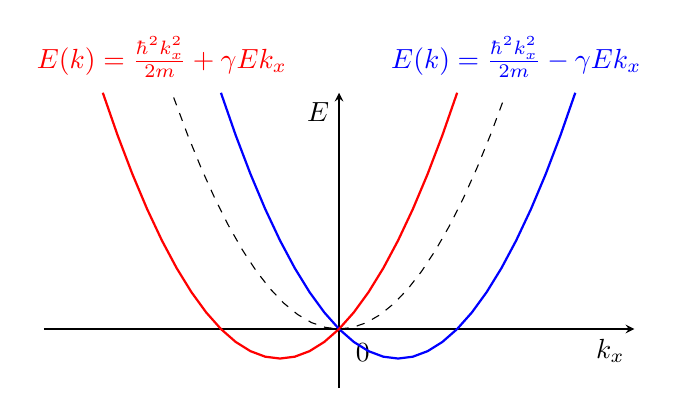
\begin{tikzpicture}[
        scale=1.5,
        >=stealth,
        ]
        % Axes
        \draw[->] (-2.5,0) -- (2.5,0) node[below left] {$k_x$};
        \draw[->] (0,-0.5) -- (0,2) node[below left] {$E$};
        \node at (0.2, -0.2) {$0$};

        % Parabolic bands
        \draw[blue, thick, domain=-1:2] plot (\x, {\x*\x - 1*\x});
        \draw[red, thick, domain=-2:1] plot (\x, {\x*\x + 1*\x});

        % Original band
        \draw[black, dashed, domain=-1.4:1.4] plot (\x, {\x*\x});

        % Labels
        \node at (1.5, 2.3) [text=blue] {$E(k) = \frac{\hbar^2 k_x^2}{2m} - \gamma E k_x$};
        \node at (-1.5, 2.3) [text=red] {$E(k) = \frac{\hbar^2 k_x^2}{2m} + \gamma E k_x$};

    \end{tikzpicture}
\end{figure}

\subsection{}
\(H\)を行列表示すると、
\begin{equation}\begin{aligned}[b]
    H = \begin{pmatrix}
        \frac{\hbar k_x^2}{2m} & \frac{1}{2}g\mu_BB+i\gamma Ek_x\\
        \frac{1}{2}g\mu_BB-i\gamma Ek_y & \frac{\hbar^2k_x^2}{2m}
    \end{pmatrix}
\end{aligned}\end{equation}
これの固有エネルギーは
\begin{equation}\begin{aligned}[b]
    0 &= \abs{H-E} = \qty(\frac{\hbar k_x^2}{2m}-E)^2-\qty(\frac{g^2\mu_B^2B^2}{4}+\gamma^2 E^2k_x^2)\\
    E &= \frac{\hbar k_x^2}{2m}\pm\sqrt{\frac{g^2\mu_B^2B^2}{4}+\gamma^2 E^2k_x^2}
\end{aligned}\end{equation}
スピンの向きに関して、
\(k_x=0\)では\(H_{SO}\)が効かないので、
スピンの向きは\(x\)方向を向いている。
低いエネルギーバンドは\(-x\)方向で、
高いエネルギーバンドは\(+x\)方向を向いている。

\(k_x\)が大きいときには\(H_{SO}\)が主に効く。
このときスピンの方向は\(y\)方向を向いていて、
\(k_x>0\)では低いエネルギーバンドでのスピンは\(+y\)方向を、
高いエネルギーバンドではスピンは\(-y\)方向を向いている。
\(k_x<0\)では逆に、低いエネルギーバンドでのスピンは\(-y\)方向を、
高いエネルギーバンドではスピンは\(+y\)方向を向いている。

\begin{figure}[h]
    \centering
    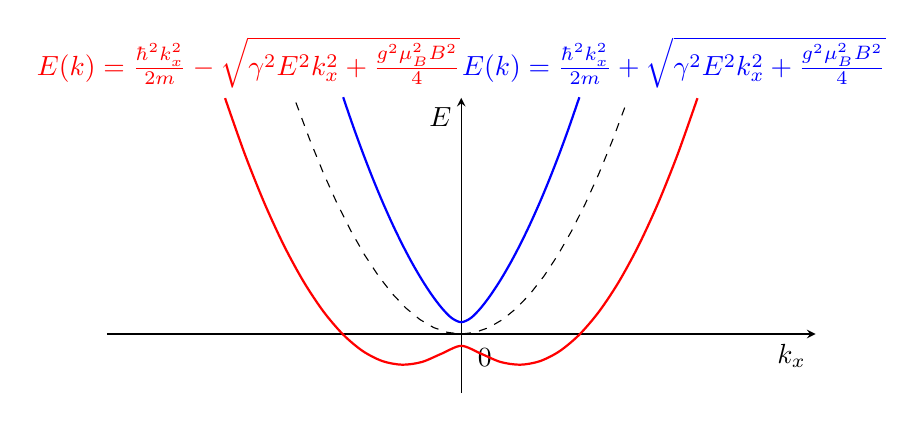
\begin{tikzpicture}[
        scale=1.5,
        >=stealth,
        ]
        % Axes
        \draw[->] (-3,0) -- (3,0) node[below left] {$k_x$};
        \draw[->] (0,-0.5) -- (0,2) node[below left] {$E$};
        \node at (0.2, -0.2) {$0$};

        % Parabolic bands with Zeeman gap
        % E(k) = k^2 +- sqrt( (alpha*k)^2 + Delta^2 )
        \draw[blue, thick, domain=-1:1, smooth] plot (\x, {\x*\x + sqrt(\x*\x + 0.01)});
        \draw[red, thick, domain=-2:2, smooth] plot (\x, {\x*\x - sqrt(\x*\x + 0.01)});

        % Original band (no SO coupling or B-field)
        \draw[black, dashed, domain=-1.4:1.4] plot (\x, {\x*\x});

        % Labels
        \node at (1.8, 2.3) [text=blue] {$E(k) = \frac{\hbar^2 k_x^2}{2m} + \sqrt{\gamma^2 E^2 k_x^2 +\frac{g^2\mu_B^2B^2}{4}}$};
        \node at (-1.8, 2.3) [text=red] {$E(k) = \frac{\hbar^2 k_x^2}{2m} - \sqrt{\gamma^2 E^2 k_x^2 +\frac{g^2\mu_B^2B^2}{4}}$};

    \end{tikzpicture}
\end{figure}

\section*{感想}
トポロジカル物性とか量子ホール効果みたいな、
スピン軌道結合による時間反転対称性を破れた系は今のところやってないので、
手で解ける例をやれて楽しかった。
この相互作用はRashbaと言われるやつかな。

\end{document}
